% Thanks to http://tex.stackexchange.com/a/30782/5645 for this
% example!
\documentclass{article}
\usepackage{amsmath}
\usepackage{mathptmx}
\usepackage{tikz}
\usepackage{pgfplots}
\usepgfplotslibrary{polar}
\usepackage{tkz-fct}
\usetikzlibrary{angles, quotes}
\usetikzlibrary{arrows.meta, arrows}
\usetikzlibrary{external}
\tikzexternalize[prefix={external/}]

\tikzset{
    export as png/.style={
        external/system call/.add={}{
            && convert -density #1 -transparent white "\image.pdf" "\image.png"
        },
    },
    export as png/.default={200},
}

\DeclareSymbolFont{symbolsb}{OMS}{cmsy}{m}{n}
\SetSymbolFont{symbolsb}{bold}{OMS}{cmsy}{b}{n}
\DeclareSymbolFontAlphabet{\mathcal}{symbolsb}
\definecolor{myblue}{rgb}{0.067,0.529,0.871}
\definecolor{mypurple}{rgb}{0.859,0.071,0.525}
\definecolor{myred}{rgb}{1.0, 0.13, 0.32}
\definecolor{mygreen}{rgb}{0.01, 0.75, 0.24}
\definecolor{myblack}{gray}{0.5}
\definecolor{mygray}{gray}{0.7}

\def\req{\protect\rotatebox{90}{$\scriptstyle=$}}

\begin{document}

\tikzset{export as png}

\tikzsetnextfilename{area-curva-polares}
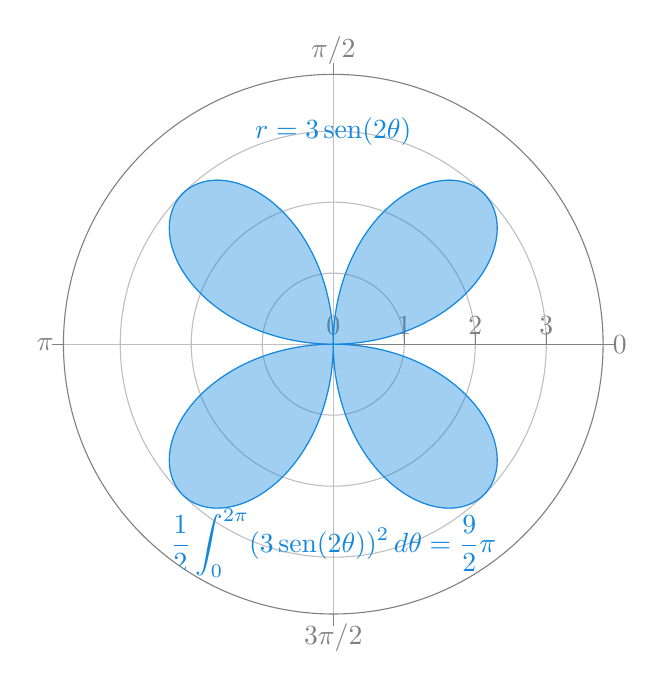
\begin{tikzpicture}
    \begin{polaraxis}[
        myblack,
        xtick={0,90,180,270},
        xticklabels = {$0$, $\pi/2$, $\pi$, $3\pi/2$},
        ymax=3.8,
        ytick={0,1,2,3},
    ]
        \addplot+ [mark=none, domain=0:360, samples=600, color=myblue, fill=myblue, opacity=0.4] {3*sin(2*x)};
        \addplot+ [mark=none, domain=0:360, samples=600, color=myblue] {3*sin(2*x)};
        \node[myblue] at (axis cs:90,3) {$r = 3\operatorname{sen}(2\theta)$};
        \node[myblue] at (axis cs:270,2.8) {$\displaystyle\frac{1}{2} \int_0^{2\pi} (3\operatorname{sen}(2\theta))^2\,d\theta=\frac{9}{2}\pi$};
    \end{polaraxis}
\end{tikzpicture}
\end{document}


